We will now present a representation of the problem which will greatly simplify the analysis of $v$ and $h$ collisions for some ball $B$, called the tiling representation. First we will define some basic definitions we need to explain the tiling representation.

\begin{definition}
  A billiard ball \emph{trajectory} $\tau(t_0, t_1)$ is the curved traced by a billiard ball $B$ between times $t_0$ and $t_1$.
\end{definition}

\begin{definition}
  A collision time $\kappa_i$ for a billiard ball $B$ is the time at which the $i$th collision occurs.
\end{definition}

To understand the basics of how the tiling representation works, imagine placing a square billiard table on the $xy$ plane. The billiard table is the unit square$[0,1]^2$. The table's edges will be the four line segments bordering the unit square. A ball will start with some initial position $\bvec{x}_0 \in [0,1]^2$ and velocity $\bvec{v}_0$. After some time, the ball will collide with an edge $e_0$ of the table at time $\kappa_1$. However, instead of thinking of the trajectory of the ball as being reflected across the line perpendicular to $e_0$ at the point of collision, we will instead reflect the original unit square $s_0$ across the edge $e_0$ to create a new square $s_1$. Now, the trajectory $\tau(\kappa_1, \kappa_2)$ of the ball after the first collision will be traced in the new square $s_1$.

In other words, the trajectory $\tau(0, \kappa_1)$ before the first collision will be confined to the original square $s_0$, and the trajectory$\tau(\kappa_1, \kappa_2)$ after the first collision will be confined to the new reflected square $s_1$. We can continue the process for each new collision. Suppose the ball collides with edge $e_1$ in square $s_1$. Then, we will create a new square $s_2$ which is a reflection of square $s_1$ across the edge $e_1$. The trajectory of the ball $\tau(\kappa_2, \kappa_3)$ after the second collision will be confined to the newest reflected square $s_2$. This process will continue on indefinitely so that the trajectory $\tau(\kappa_j, \kappa_{j+1})$ will be confined to the square $s_j$, where square $s_{j+1}$ is generated by reflecting square $s_{j}$ across the edge $e_{j}$ which is collided with at time $\kappa_j$.

Figure \ref{fig:tiling} shows an example trajectory which is created using this tiling process. In essence, the tiling representation reflects a table about each of its four sides. These reflections will perform the same process, eventually tiling and completely filling the $xy$ plane. The trajectory of particular billiard ball can then be traced through the tiling in the $xy$-plane, as seen in figure \ref{fig:tiling}.

\begin{figure}
  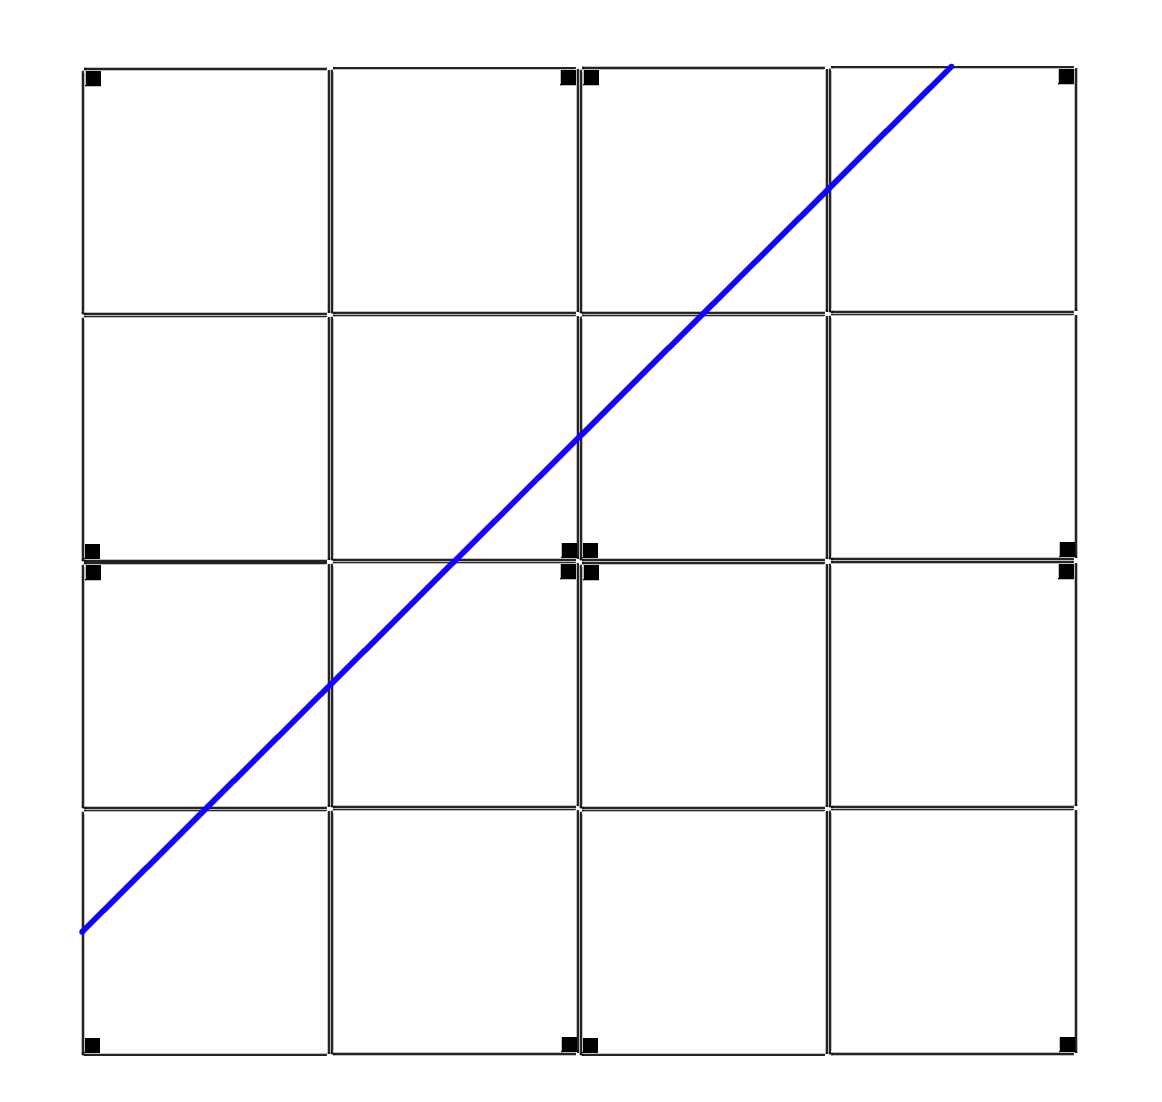
\includegraphics[width=3in]{tiling.png}
  \caption{\label{fig:tiling}Example of Tiling Billiard Tables}
\end{figure}

A couple of interesting observations can be made:

\begin{itemize}
  \item The combined trajectory $T = \{\tau(0, \kappa_1), \tau(\kappa_1, \kappa_2), \tau(\kappa_2, \kappa_3), \ldots \}$ of a ball creates a ray in the $xy$ plane.
  \item All $v$-collisions happen exactly when the combined trajectory $T$ intersects with the integer vertical lines $x = k$ where $k \in \mathrm{Z}$. The same can be said of $h$-collisions and integer horizontal lines $y = k$ for $k \in \mathrm{Z}$.
\end{itemize}

We can formalize and prove each of these observations in turn:

\begin{theorem}
  The combined trajectory $T = \{\tau(0, \kappa_1), \tau(\kappa_1, \kappa_2), \ldots\}$ of a billiard ball is a ray in the $xy$ plane under the tiling representation.
  \label{theorem:straight-line}
\end{theorem}
\begin{proof}
  We need to show that all trajectories $\tau(0, \kappa_1), \tau(\kappa_1, \kappa_2), \ldots$ which constitute the combined trajectory lie on a single line. We know that trajectories $\tau(\kappa_i, \kappa_{i+1})$ are line segments because the velocity of the billiard ball only changes during a collision. Thus, we just need to show that each trajectory $\tau(\kappa_i, \kappa_{i+1})$ lies on the same line, i.e. that $\tau(\kappa_i, \kappa_{i+2})$ is a line segment for all $i \in \mathrm{Z}$.

  We will show this by analyzing the change in trajectory at time $\kappa_i$. We know that at any time $t \in (\kappa_{i-1}, \kappa_i)$, the billiard ball will be on the line segment defined by the trajectory $\tau(\kappa_{i-1}, \kappa_i)$. This trajectory makes an angle $\theta$ with the edge $e_i$ which the billiard ball collides with at time $\kappa_i$. Moreover, we know that after colliding with $e_i$, the outgoing angle of the trajectory is equal to the incoming angle $\theta$ by our definition of collision.

The velocity is reflected about the line perpendicular to $e_i$ at the point of collision, but the angle of the trajectory $\tau(\kappa_i, \kappa_{i+1})$ makes with $e_i$ remains the same. Thus, when square $s_{i}$ is reflected about $e_i$, the resulting trajectory in $s_{i+1}$ makes an angle of $\theta$ with $e_i$. Figure \ref{fig:straight-line-angle} shows this process graphically.

\begin{figure}
  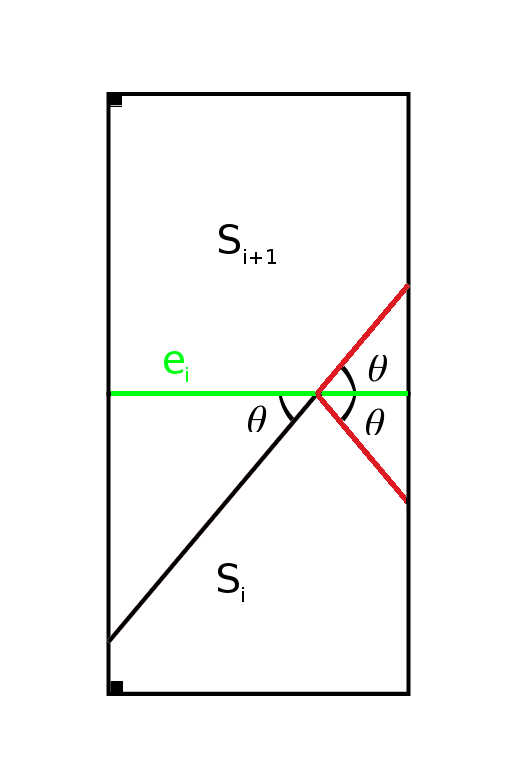
\includegraphics[height=2in]{tiling_straight_line_proof.png}
  \caption{\label{fig:straight-line-angle}Trajectories $\tau(\kappa_{i-1}, \kappa_i)$ in $s_i$ and $\tau(\kappa_{i}, \kappa_{i+1}$ $s_{i+1}$ forming a line segment}
\end{figure}

It is clear that the angles that $\tau(\kappa_{i-1}, \kappa_i)$ and $\tau(\kappa_{i}, \kappa_{i+1}$ make with $e_i$ are both $\theta$. Since both of these trajectories are already line segments, we see that the union of the two trajectories is also a line segment because both trajectories lie on the same line. Thus, we see that all trajectories $\tau(\kappa_j, \kappa_{j+1})$ for all $j \in \mathrm{Z}$ lie on the same line, which completes the proof.
\end{proof}

\begin{theorem}
  Let $t_{v, k}$ be a time when the combined trajectory $T$ intersects with some integer vertical line $x = k$ where $k \in \mathrm{Z}$. We must have $\kappa^v_k = t_{v, k}$, where $\kappa^v_k$ is the time at which the $k$th $v$-collision occurs.

  Similarly, let $t_{h, k}$ be a time when the combined trajectory $T$ intersects with some horizontal vertical line $y = k$ for $k \in \mathrm{Z}$. Then, $\kappa^h_k = t_{h, k}$.
\end{theorem}
\begin{proof}
  The proof of the first statement is exactly analogous to the proof of the second statement, so we will only prove the theorem for $\kappa^v_k = t_v$.

  Recall that in the tiling representation, whenever the billiard ball collides with an edge $e_j$, a new square $s_{j+1}$ gets reflected across $e_j$. It is clear that $e_j$, if it is a horizontal edge, lies on some integer horizontal line $y = c$ where $c \in \mathrm{Z}$. Alternatively, if $e_j$ is a vertical edge then it lies on some integer vertical line $x = c$ where $c \in \mathrm{Z}$. Thus each $\kappa_j$ corresponds to when the combined trajectory $T$ intersects with some integer vertical or integer horizontal line.

  It is also clear that the billiard ball cannot make a $v$-collision at time $t$ unless the combined trajectory $T$ intersects with an integer vertical line at time $t$ as well. Therefore, we see that $v$-collisions occur exactly when $T$ intersects with an integer vertical line.

  We know that $T$ traces a ray in the $xy$ plane by theorem \ref{theorem:straight-line}. By assumption, this ray starts in the unit square $[0,1]^2$ and has an angle between $0$ and $\pi/2$ with the horizontal. Thus, the first $v$-collision occurs when $T$ intersects $x = 1$, the second $v$-collision occurs when $T$ intersects $x = 2$, and the $k$th $v$-collision occurs when $T$ intersects $x = k$.

  However, we know that the $k$th $v$-collision occurs at time $\kappa^v_{k}$ by definition, and that the $t_{v, k}$ is the time when $T$ intersects with $x = k$. Therefore, we see that $\kappa^v_{k} = t_{v, k}$.
\end{proof}

We now see that we can represent the combined trajectory $T$ of a billiard ball as a ray in the plane. We can define the line which the ray lies on as $y = mx + y_0$, where $m$ is the slope of the line and is given by $m = \frac{\bvec{v}_y}{\bvec{v}_x}$ and $y_0$ is the $y$-intercept which can be determined by $\bvec{x}_0$ by solving for $\bvec{x}_y = m \bvec{x}_x + y_0$. This line represents the entire combined trajectory, and also determines all possible collision sequences for a particular billiard ball, since $v$-collisions happen when $x$ is an integer and $h$-collisions happen when $y$ is an integer.
